%                      Code_Saturne version 1.3
%                      ------------------------
%
%     This file is part of the Code_Saturne Kernel, element of the
%     Code_Saturne CFD tool.
% 
%     Copyright (C) 1998-2007 EDF S.A., France
%
%     contact: saturne-support@edf.fr
% 
%     The Code_Saturne Kernel is free software; you can redistribute it
%     and/or modify it under the terms of the GNU General Public License
%     as published by the Free Software Foundation; either version 2 of
%     the License, or (at your option) any later version.
% 
%     The Code_Saturne Kernel is distributed in the hope that it will be
%     useful, but WITHOUT ANY WARRANTY; without even the implied warranty
%     of MERCHANTABILITY or FITNESS FOR A PARTICULAR PURPOSE.  See the
%     GNU General Public License for more details.
% 
%     You should have received a copy of the GNU General Public License
%     along with the Code_Saturne Kernel; if not, write to the
%     Free Software Foundation, Inc.,
%     51 Franklin St, Fifth Floor,
%     Boston, MA  02110-1301  USA
%
%-----------------------------------------------------------------------
%

%%%%%%%%%%%%%%%%%%%%%%%%%%%%%%%%%%
%%%%%%%%%%%%%%%%%%%%%%%%%%%%%%%%%%
\section{Discr\'etisation}
%%%%%%%%%%%%%%%%%%%%%%%%%%%%%%%%%%
%%%%%%%%%%%%%%%%%%%%%%%%%%%%%%%%%%

La figure \ref{Base_Itrmas_fig_geom} rappelle les diverses d\'efinitions g\'eom\'etriques
pour les faces internes et les faces de bord. 

\begin{figure}[h]
\parbox{8cm}{%
\centerline{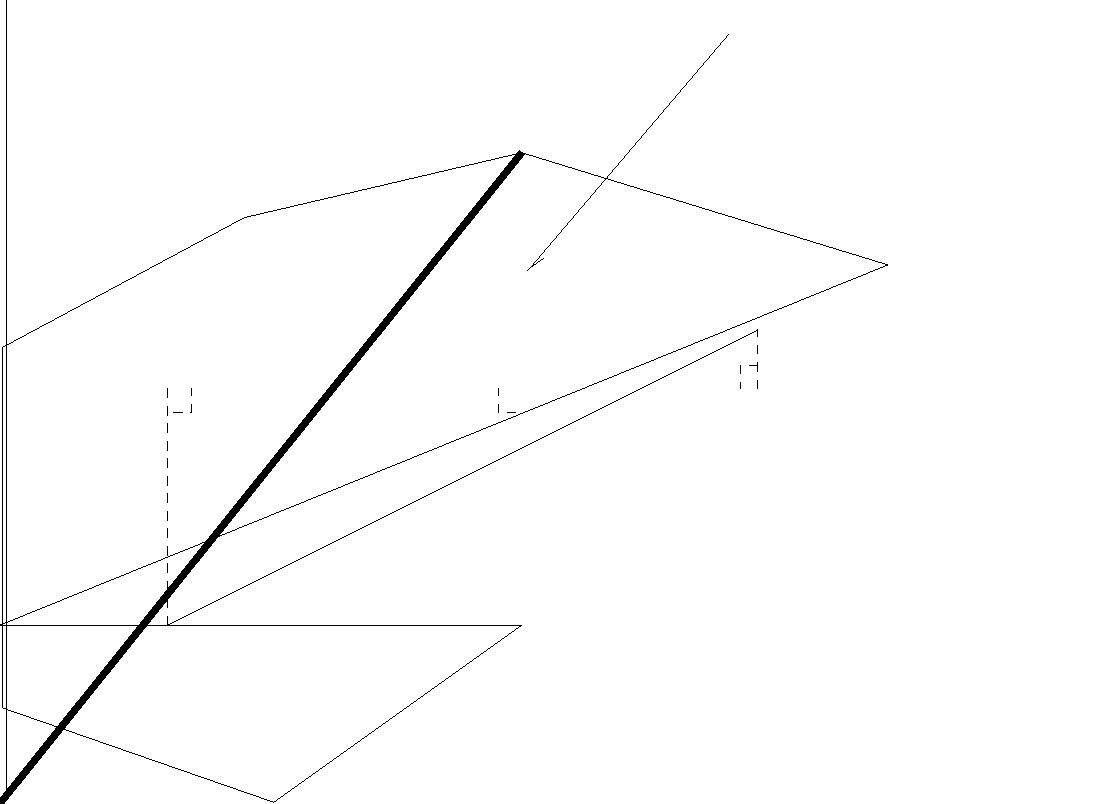
\includegraphics[height=4cm]{../Base/Itrmas/Images/facette.pdf}}}
\parbox{8cm}{%
\centerline{
\includegraphics[height=4cm]{../Base/Itrmas/Images/facebord.pdf}}}
\caption{\label{Base_Itrmas_fig_geom}D\'efinition des diff\'erentes entit\'es
g\'eom\'etriques pour les faces internes (gauche) et de bord (droite).}
\end{figure}


\subsection{Calcul sans reconstruction des non orthogonalit\'es}
Pour les faces internes, on \'ecrit simplement :
\begin{equation}
\label{Base_Itrmas_eq_intssrec}
-\Delta t_{\,ij}(\grad_f P)_{\,ij}\,.\,\vect{S}_{\,ij}=
\frac{\Delta t_{\,ij}S_{\,ij}}{\overline{I^\prime J^\prime}}(P_I-P_J)
\end{equation}

Pour les faces de bord, on \'ecrit :
\begin{equation}
\label{Base_Itrmas_eq_brdssrec}
-\Delta t_{b_{ik}}(\grad_f P)_{\,b_{ik}}\,.\,\vect{S}_{\,b_{ik}}=
\frac{\Delta t_{\,b_{ik}}S_{\,b_{ik}}}{\overline{I^\prime F}}
\left((1-B_{b,ik})P_I-\var{INC}\times A_{b,ik}\right)
\end{equation}

Les pas de temps aux faces $\Delta t_{\,ij}$ et $\Delta t_{\,b_{ik}}$ sont calcul\'es
par interpolation par les sous-programmes \fort{viscfa} (cas isotrope,
\var{IPUCOU=0}) ou \fort{visort} (cas anisotrope, \var{IPUCOU=1}).


\subsection{Calcul avec reconstruction des non orthogonalit\'es}
Plusieurs discr\'etisations peuvent \^etre propos\'ees pour le traitement des
non orthogonalit\'es. Celle retenue dans le code est issue des premiers tests
r\'ealis\'es sur le prototype, et fait intervenir non seulement le pas de temps
interpol\'e \`a la face, mais aussi les pas de temps dans chaque
cellule. Il
serait sans doute bon de revenir sur cette \'ecriture et \'evaluer d'autres
solutions. La forme utilis\'ee pour les faces internes est :
\begin{multline}
\label{Base_Itrmas_eq_intavcrec}
-\Delta t_{\,ij}(\grad_f P)_{\,ij}\,.\,\vect{S}_{\,ij}=
\frac{\Delta t_{\,ij}S_{\,ij}}{\overline{I^\prime J^\prime}}(P_I-P_J)\\
+(\vect{II}^\prime-\vect{JJ}^\prime).\frac{1}{2}\left[
\Delta t_I(\grad P)_I+\Delta t_J(\grad P)_J\right]
\frac{S_{\,ij}}{\overline{I^\prime J^\prime}}
\end{multline}

Pour les faces de bord, on \'ecrit :
\begin{equation}
\label{Base_Itrmas_eq_brdavcrec}
-\Delta t_{\,b_{ik}}(\grad_f P)_{\,b_{ik}}\,.\,\vect{S}_{\,b_{ik}}=
\frac{\Delta t_{\,b_{ik}} S_{\,b_{ik}}}{\overline{I^\prime F}}
\left[(1-B_{b,ik})(P_I+\vect{II}^\prime.(\grad P)_I)-\var{INC}\times A_{b,ik}\right]
\end{equation}

